\documentclass{article}
\usepackage[utf8]{inputenc}
\usepackage{amsmath}
\usepackage{algorithm}
\usepackage{algorithmic}
\usepackage{tikz}
\usepackage{pgfplots}
\usepackage{multirow}


\title{Comparison of SSSP algorithms}
\author{Patrick Vickery }
\date{August 2017}

\begin{document}

\maketitle

\section{Introduction}
This paper discusses the single source shortest path problem (SSSP) and compares multiple algorithms against each other. The algorithms of interest can solve the general case where graphs can have negative edges. If there is a negative cycle in the graph, the algorithms terminate and notifies the user. When all of the edges are non-negative, we can compare the runtimes of the general algorithms and Dijkstra's to see how much longer it takes to allow negative edges, even when they are not present. A random graph generator was constructed to create large batches of graphs which were used to compare the algorithms average runtimes. Implementation details of the algorithms, data structures and generator are discussed then the results are compared.

\subsection{Notation}
\begin{itemize}
\item $G=(V,E)$ is a graph with vertices $V$ and edges $E$
\item $n,m = \lvert V \rvert, \lvert E \rvert$
\item $s$ is the source of the search problem
\item $uv\in E$ is the edge from $u$ to $v$
\item $c_{uv}$ is the cost of the edge $uv$. If the edge does not exists, $c_{uv}= \infty$
\item $d_i$ is the current minimum cost from $s$ to $i \in V$
\item $deg(v)$ is the degree of vertex $v$
\end{itemize}

\subsection{Definitions}
\begin{itemize}
\item Induced subgraph by $V' \in V$ is the subgraph of $G$ where the vertices are $V'$ and the edges are $uv, u\in V' v\in V'$.
\item k-claw is a bipartite graph with 1 vertex in one partition and $k$ vertices in the other.
\item Single source shortest path (SSSP) problem - Given a graph with nonnegative edges and a source, find the shortest path tree from the source.
\item General SSSP (GSSSP) - Given a graph with nonnegative cycles and a source, find the shortest path tree from the source.
\item DAG: Directed acyclic graph
\end{itemize}
\section{Motivation and Applications}
\subsection{SSSP}
Graphs can be used to represent a wide variety of real work networks such as distance between locations which are often used for resource transportation. SSSP algorithms can be used on these networks to find the shortest route from a source to a destination (or a source to all other locations). This can either optimize the time that a package travels through a networks or the distance that is travelled.\\
Some practical applications are:
\begin{itemize}
	\item IP/TCP - What is the quickest way to send data from one computer to another?
	\item Transportation of Resources - Sending inventory from factories to various locations.
	\item GPS Route - Finding quickest way from A to B. 
\end{itemize}

\subsection{GSSSP}
If negative edges are allowed, the previous networks no longer make sense. We can not travel from A to B and loose time or move a negative distance. Instead, these networks can represent economic systems such as the foreign currency exchange market (forex). 

\subsubsection{Forex}
Vertices represent our various currencies and directed edges $uv$ represent the negative natural logarithm of the exchange rate from currency $u$ to currency $v$. The log is used to map the exchange rate, a positive real, to all reals in order to use negative edges. This also changes the way we think of this network; previously, the currency is multiplied by the conversion rate to find the new amount, but now the edge weights represent the cost of that exchange and, therefore, is added which allows GSSSP algorithms to be run. They start at one currency to find the best route to convert money to another currency. If we find a negative cycle, we have found an arbitrage that can be used to capitalize off of. An arbitrage is when the difference in the buy/sell prices between 2 vendors is large enough to make a profit by buying from one vendor and selling directly to the other. \\
For example: There are 2 vendors $X_1$ and $X_2$ that are both buying and selling CAD, Canadian currency, and USD, American currency. Conversion rates, represented as From/To, are:
\[X_1: CAD/USD = 0.7, USD/CAD = 1.3\]
\[X_2: CAD/USD = 0.8, USD/CAD = 1.2\]
Once mapped using $-log(x)$, the values are:
\[X_1: CAD/USD = 0.36, USD/CAD = -0.26\]
\[X_2: CAD/USD = 0.22, USD/CAD = -0.18\]
These values represent the percentage of the amount converted that is 'spent' for that exchange. Negative values then represent the percentage of units of currency gained. A negative cycle would allow us to continously make profit as long as it exists. In the above example, if we start with $100CAD$, we can exchange it, using $X_2$, to get $80USD$. Then we exchange it again using $X_1$, to get $104CAD$, a net profit of $4CAD$.


\section{Algorithms}

\subsection{Dijkstra}
Dijkstra \cite{Dijkstra} is a greedy algorithm that finds the SSSP tree. It is initialized to just be the source vertex and 1 edge and node is repeatedly added to the shortest path tree until the tree is complete. There is no backtracking in this algorithm, so if an edge/node pair is added, it is in the final SSSP tree. This can also be desribed by it's invarient: the shortest path tree, while being constructed, is always the shortest path tree of the subgraph induced by the nodes in the SSSP tree. This algorithm is rather simple and runs quickly, $O(n \cdot lg(n))$, but does not always produce the correct answer if negative edges are included.

\subsection{Example}
To compare some of the algorithms, we present the graph in Figure 1 to show how different algorithms run on it and how Dijkstra's algorithm fails to produce the correct answer.
\begin{figure}
	\centering
	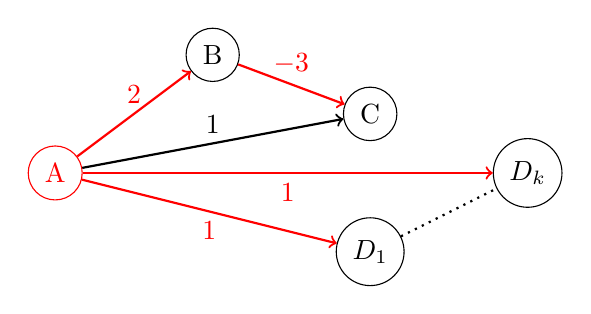
\begin{tikzpicture}
	\node[draw,circle,color=red] (A) at (0,-1.5) {A};
	\node[draw,circle] (B) at (2,0) {B};
	\node[draw,circle] (C) at (4,-.75) {C};
	\node[draw,circle] (Dk) at (6,-1.5) {$D_k$};
	\node[draw,circle] (D1) at (4,-2.5) {$D_1$};
	
	\draw [->, thick, color=red] (A) edge node[above] {$2$} (B);
	\draw [->, thick] (A) edge node[above] {$1$} (C);
	\draw [->, thick, color=red] (B) edge node[above] {$-3$} (C);
	
	\draw [->, thick, color=red] (A) edge node[below] {$1$} (D1);
	\draw [->, thick, color=red] (A) edge node[below] {$1$} (Dk);
	\draw [dotted, thick] (D1) edge node[below] {} (Dk);
	

	\end{tikzpicture}
\caption{Graph with k-claw from $a$ to $d_i, 1 \leq i \leq k$. Shortest path tree from source $A$ is highlighted red}
\end{figure}
Dijkstra's algorithm starts with the SSSP tree as $T = \{\{s\}, \{\}\}$. Next, the shortest edges from $s$ are added: $ac$ and $ad_i, 1 \leq i \leq k$. Finally, the only other edge available is $ab$ so it is added, and all vertices are reached, so the algorithm terminates. However, this is not the correct shortest path tree which is shown in red. Since Dijkstra's algorithm does not account for negative edges, $bc$ was not ever considered to be in the shortest path tree since it is 'hidden' behind $ab$ which is selected last. If negative edges are present, other algorithm are needed instead.

\subsection{Relaxation}
Relaxation is a technique often used when negative edges are allowed to check if $d_i$ can be reduced by changing the parent of $i$. Relaxation is applied repeatedly on all vertices (or edges) until an answer is found. If negative cycles are present, there is no convergence on an answer since a path cost can always be reduced by using the negative cycle another time.

Since we are looking for the shortest path to each vertex, the number of edges from the source to any other vertex must be at most $n-1$. If not, then it is not a path but a trail (vertices can repeat but edges cannot) and a trail would only have a lower cost if a negative cycle is present. Therefore, once we relax every edge $n-1$ times, we must have found a solution if no negative cycles are present.

\subsection{Bellman-Ford}
The Bellman-Ford algorithm \cite{BF, BF 2} uses relaxation on all vertices $n-1$ times to find the solution. It initialized $\forall_{i\in V-\{s\}} d_i = \infty, d_s = 0$. If we look how it runs on Figure 1, the first iteration makes the following changes: $a_b = 2, a_c = 1, d_{i}, 1 \leq i \leq k = 1$. The second iteration makes a single change, $d_c = -1$. At this point no more changes will be made since the shortest path tree has been found. However, Bellman-Ford does not accound for this and will continue to try to relax the graph $k+1$ more times without making any changes.

\subsection{SPFA}
As we saw above, there will be many instances where we will end up doing unnecessary relaxations when using Bellmand-Ford. They can be avoided by only relaxing edges from vertices that have been relaxed during the current or previous iteration of relaxation over $n-1$. SPFA would run the same way as Bellman-Ford on Figure 1, but would terminate after the 3rd iteration since it was found that no more changes can be made.

This is commonly called Shortest Path Fast Algorithm and credited to Fanding Duan \cite{SPFA}. However, it was first discovered by Jin Y. Yen in in 1969 \cite{Yen2} and published in his book \textit{Shortest Path Network Problems} shortly after his dissertation at Berkeley and publication of \cite{Yen1}. It was not named in his book but is sometimes called Yen's 1st improvement to the Bellman-Ford algorithm. His second improvement is even more interesting.

\subsection{Yen's Improvement to Bellman-Ford}
Yen \cite{Yen Decomposition} used decomposition to split a graph into 2 edge-disjoint DAGs: $G^+$, $G^-$. The idea was likely inspired by the Hu-Torres decomposition \cite{Hu, Hu Torres} which solves SSSP for edge-distinct subsets and combines the results. The DAGs are created by uniquely labeling each vertex arbitrarily from $1$ to $n-1$ and labeling the source $0$. Then, $G^+$ only contains edges $uv$ where the label of $u$ is less than the label of $v$ and $G^-$ contains the rest (label of $u$ is greater than the label of $v$). For example, on adjacency matrices $G^+$ and $G^-$ could be the upper and lower triangular of the origonal matrix. This allows for relaxation to be used slightly different from before.  Instead of relaxing all possible edges at once (Bellman-Ford) or relaxing 1 edge at a time (SPFA), relaxation is applied to all edges in each DAG, but in a very specific order: minimum absolute label distance from the source. in $G^+$ and minimum number of edges from the vertex labelled $n-1$. A single iteration of relaxation is applied to each DAG 1 at a time until both DAGs have been relaxed $n-1$ times since the shortest path tree has n-1 edges.
\subsection{Label correcting improvements}
Label correcting algorithms can be used on queue-based SSSP problems (such as Bellman-Ford or Yen's improvement) to order the queue in a more optimal manner.

\subsubsection{Bertsekas}
\cite{Bertsekas1, Bertsekas2} proposed 2 methods of reordering the queue: \textit{Small Label First} and \textit{Large Label Last}. Instead of adding vertices, $v$, to the back of the queue every time:
For \textit{Small Label First}, if $deg(v) < deg(\text{front})$ add $v$ to the front of the queue.
For \textit{Large Label Last}, let $s = \sum_{\forall v \in V}deg(v) /\|V\|$ and $f$ be the first vertex in the queue. Add $v$ to the end of the queue. While $f > s$ move $f$ to the back of the queue.\\
These methods can be combined with the threshold algorithm and, as shown in \cite{Bertsekas1}, work efficiently in practice.

\subsubsection{Pape}
\cite{Pape} modified the queue such that any element that has been visited before is added to the front of the queue. \cite{Hao} also showed that this method could be combined with with Bertsekas method above. 

\section{Implementation details}
\subsection{Data Structures}
\subsubsection{Graph Generics}
There are currently 2 graph implementations: adjacency matrix and adjacency lists, that share a parent class GraphADT. GraphADT is a virtual, abstract class. By using pointers to GraphADT, we can consistently refer to the inherited classes using the same type. This allows easy creation of a containers with different graph types. It also simplifies the algorithms and the generator so that they don't care what type of graph they are working with.
\subsubsection{Visualization}
The export dot method allows for the graphs to be viewed visually. The graph image displays edge weights, node labels and each edge indicates if it is directed by having an arrow instead of a line. In order to highlight a shortest path tree another, optional argument is included. This allows a set of edges (or rather, edge indicies) that will be highlighted on top of the origonal graph. Instead of printing all edges then printing edges in the shortest path tree a second time, now highlighted, a set is used to store the edges to provide quick search time. While printing each line to the dot file, check if the current edge is in the set, and if so, color it red. 
\subsubsection{Convertor}
A converter was created to take a GraphADT pointer, referring to some unknown graph type, and convert it to another graph implementation. This preserves the structure of the graph, edges and vertices, which allows for runtime comparisons between implementations.
\subsubsection{Star Representation}
I found a very interesting graph implementation that I had never seen before and is a good replacement for adjacency lists. \\
The star representation \cite{Star} uses an array to store the edges, like the adjacency matrix, but only uses $O(n+m)$ space, like the adjacency list. There are 2 main types of the star representation: forward and reverse. They provide an efficient way to access incoming and outgoing edges respectively but can also be combined to quickly access both incoming and outgoing edges. \\
First, number the arcs from $1$ to $m$ and create a $3*m$ array that represents the tail, head, and weight of each edge. We use tail($i$), head($i$), and weight($i$) to access the attributes of the $i$'th edge. Next we create a $1*n$ array of pointers. For the forward representation, each pointer pointer($i$) points to the smallest numbered edge leaving $i$ and the $3*m$ array is sorted by the tail column. For the backwards representation, each pointer pointer($i$) points to the smallest numbered edge entering $i$ and the $3*m$ array is sorted by the head column. \\
If we want to have easy access to all incoming and outgoing edges, we can use both the forward and reverse star representation but will have duplicate information. We can use the compact star representation which reduces the space needed. It contains all data from the forward representation ($1*n$ array of pointer and $3*m$ array of edges sorted by tail) but instead of duplicating the $3*m$ matrix and sorting by head, we can create a $1*n$ array of pointers as before but they will point to a new $1*m$ array which represents the vertex numbers sorted by head. This give us access to the array sorted by head an tail which allows access to both forward and reverse representations with only $n+m$ additional entries from a single representation.



\subsection{Generator and Builder}
The Erdős–Rényi random graph models generate graph by specifying the number of edges or the probability of each edge being added. To do this, a random number generator that creates a random number in a specified range is included. The different models required different types of numbers so a template was used to return floats, for probability, and unsigned integers for set edges. In order to select a set number of edges, each randomly selected edge must be unique. We could repeatedly randomly select an edge until we find a unique edge to add. However, this could take a very long time so instead I used reservoir sampling, which selected distinct values from an input set. In order to be able to select a wide variety of edges, the input set is passed as a parameter. This makes it easier to generate edges for acyclic graphs since the potential edges are not numbered from 0 to $m-1$. In short, when choosing $k$ unique elements from a set of $n$ elements, first select the first $k$ elements in the set and for each remaining element add it to the subset with some probability and replace an element in the subset. This way each element has equal probability of being selected. 

To generate different types of graph such as acyclic or self-loop, we need to find the potential edges to be used. A diagonal offset is used account for the restricted edges, and the remaining potential edges are sent to reservoir sampling for the set edge model, or are used directly for the probabilistic model. To add edges given a probability, a random float between 0 and 1 is compared to determine whether an edge is added. 

Finally, for generating edge weights, a method sets the range and randomly sets the weight for each existing edge. Therefore it must be called after the edges have been created. To create directed edges, create an acyclic graph and 'reflect' the edges afterwards. If the directed edge is to be weighted, it must reflected after the weights are set since, otherwise, the each direction of each edge are not guarenteed to be the same.

\subsubsection{Algorithms}
I had to create a unique queue for SPFA (and Pape) so I used a deque to hold the contents and dequeue items from and a set to check if an item is in the queue. For Dijksta's, I had to create a priority queue using the distance from the source as the key. STL and Boost both do not allow elements in a priority queue to be updated after insertion so how the elements are inserted is very important. Vertices, $v$, are only added if they are a neighbour of the current node, $c$ and the cost to $v$ will be reduced by setting $c$ as the parent. \\
I created an SSSP template to act as the interface for all of the algorithms. It is a variatic class that takes an unknown number of different algorithms types and a single graph implementation. All algorithms are run on this graph and their times are recorded. The user can specify if the want to time the results and, if so, can call a getter method to get the results. I decided to have SSSP algorithms return a set of edge indices in the shortest path tree.  I used boost:optional here to represent a vertices parent in the shortest path tree since all vertices start with no parent and even afterwards some vertices may not have been discovered (ex. disconnected graph or not reachable from the source). Then, I changed the export dot functions to take the set as a parameter and, while printing each edge to the dot file, I check if edge is in the set. This way, I can check if each edge is in the set in constant time to print a graph where the shortest path tree is coloured red. Since multiple algorithms were being run and tests, I created a method that checks if all shortest-path trees are equivelent and, if not, notifies the user of the error.
 
 
\subsubsection{Timer}
Finally, the timer needed to repeatedly generate graphs of specified parameters so a builder is accepted as a parameter. The user specifies the number of test cases and the timer generates graphs (using the builder) and runs SSSP with all algorithms on them. SSSP records the results of all algorithms on a single graph so timer collects, averages and returns those times.

\section{Timeline}

\subsection{Algorithm Research}
I started by reviewing Bellman-Ford and than began searching for papers on Shortest Path Fast Algorithm by Fanding Duan and, seperately, Jin Yen. "Shortest Path Network Problem" bv Yen covers SPFA (although it was not named by Yen) and 2 implementations of another improvement of Bellman-Ford. The improvement, referred to as Yen's 2nd improvement to Bellman-Ford, uses decomposition to solve SSSP. 

I also looked into label correcting algorithms which change the insertion position of the queue to optimize the main algorithm. Some would use the degree to either insert an item to the front or the back of the queue. Another check if the inserted element has been visited before and, if so, added it to the front of the queue. These 2 types of label-correcting algorithms, using degrees and 'visited', could be combined.

\subsection{Review C, Learn C++}
Although I started planning the design of the generator, I needed to review some C and learn C++. The main concept that I needed to learn was templates so I started to read "Modern C++ Design" by Andrei Alexandrescu. I focused on Policy Programming Design (which is similar to strategy design but with templates). I decided to use the boost template library to suppliment STL for additional features. One feature that useful was boost's optional template. I decided to use it to indicate that no such edge exists in a AdjacencyMatrix. I chose not to use the Boost Graph library since it was not a header only library (making it a more difficult dependency) and it did not include the ForwardStar/CompactStar implementation which I wanted to include when comparing runtimes.

I started programming by creating an AdjacencyMatrix as my first graph implementation. It was very simple and only added edges and nodes and set edge weights. I wanted to be able to generate different graph implementations (AdjacencyList and Compact Star), so I implemented an abstract class for graphs to inherit from in order to use run-time polymorphism. The next graph I implemented was adjacency list for sparse graphs. 

\subsection{Graph Generator}
I found that there is a common model called the Erdős–Rényi model which has 2 similar implementations. One of which sets the number of edges which required a way to select a unique subset of edges from all of the possible edges. I did some research and found that reservoir sampling would be a good solution. 

For the random graph generator, I needed to create a random number generator, and since I decided to start with the set edge Erdős–Rényi model, I only need the number generator to random unsigned integers within a specified range. Next, I implemented reservoir sampling to finish a rough version of the first Erdős–Rényi model. After I was able to generate a very basic graph, I wanted to be able to view it to check the results so I created functions to print the adjacency matrix to the console and to a graphviz dot file that can be converted into a postscript image. I, unfortunately, created duplicate code for the exportdot functions since they all worked the same way for each ADT. Next I added acyclic and directed parameters to the graph generator.

Next, I updated my random number generator to use templates to decide the return type at compile time. This allowed random floats between 0 and 1 for the probabilities as well as random naturals for reservoir sampling.

Next, I needed to generate weights between a specified range so I updated my random number generator to allow random floats between 0 and 1 for the probabilities as well as random naturals for reservoir sampling. I could've created another function to generate floats instead of unsigned integers, however I decided to create my first template class to decide the return type at compile time. I also anticipated that I might need to change the random distributions later on when trying to generate graphs nonnegative cycles. Some distributions might, on average, create less negative cycles than others. A distribution that skews toward the left (distribution mean is moved right) would likely be a good fit since (large) positive numbers would occur more often than (small) negative values and therefore likely not have long chains of negative edges. This would be helpful to reduce the number of negative cycles that I would have to correct. This is because SSSP algorithms with negative edges must not have any negative cycles so the graphs have to be changed to break any negative cycle.

\subsubsection{Builder}

I wanted to be able to create an nested builder but was not able to with the abstract data type. Instead, a seperate class was created to generate graph. It helps to create default parameters, easily choose between both Erdős–Rényi models, and set arguments in any order. The builder returns a GraphADT pointer to some graph implementation. Since I want to be able to compare different types of graphs (and how the algorithms run on them) I need to be able to convert graphs to different types. Next, I created a graph convertor to copy a graph into a different implementation within SSSP so the algorithms could run on all implementations all within SSSP. Using a builder also prevents the user from making mistakes when dealing with undirected, weighted graph. Since undirected graphs are symmetrical (when looking at adjacency matrix), an acyclic graph is generated and then reflected across the diagonal. The builder makes sure that all steps are applied in the correct order so a user doesn't create an undirected edges where $c_{uv} \neq c_{vu})$.

\subsection{Algorithms}
At this point I had everything ready to start working on the SSSP algorithms that find the shortest path tree. I started with the Bellman-Ford algorithm and then Pape's label correcting improvement. Next, I wanted to be able to visually confirm the results so I created a graphviz dot file export method for graphs. Once they were partially completed, I created a SSSP template class to use compile time polymorphism. I was able to finish the 2 algorithms at this point since I was quickly able to print results and find where mistakes were being made. Next, I changed SSSP to become a variatic template. This was my first time using variatic templates so I had to spend some time researching how they are implemented. Once I finished researching variatic templates, I figured out that recursion is used to 'unroll' the ellipsis arguments. I changed SSSP so multiple algorithms could be run at once. This way I could compare results to make sure they were both returning valid answers and, if not, identifying where they differ. Next, I began working on SPFA and was able to use the SSSP template to find any mistakes.

\subsection{Timing}
At this point, I began working on timing my results. I had to update SSSP to time each individual algorithm. Once a single algorithm could be timed, I switched to a  variatic template run multiple algorithms on the same graph. After, I wanted to be able to generate many graphs to find the average time for each algorithm and how it changed with different graph types. The tester specifies the number of graphs to be generated and, as expected, the results are more consistent when the number of trials is high.


\section{Results}
In the figures below, average runtimes were found by generating 1000 DAGs each with 100 vertices and $100\cdot t, 2 \leq t \leq 4800$ edges. Each algorithm was run on every graph so find the average runtimes with a varying number of edges.

\begin{figure}
	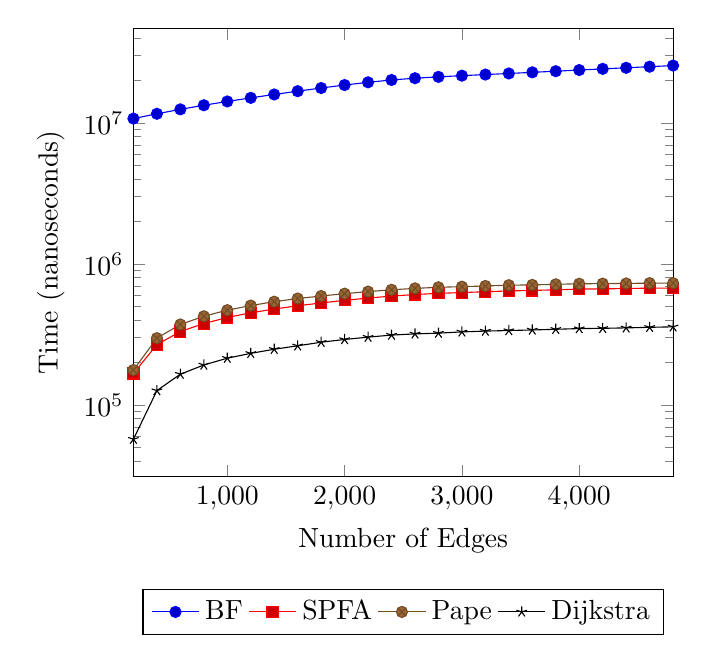
\begin{tikzpicture}
	\begin{axis}[
	ylabel={Time (nanoseconds)},
	xlabel={Number of Edges},
	ymode=log,
	xmin=200, xmax=4800,
	legend style={at={(0.5,-0.25)},
		anchor=north,legend columns=-1},
	]
	%Bellman-Ford
	\addplot+[sharp plot] coordinates
		{(200, 10736436) (400, 11613544) (600, 12481691) (800, 13348950) 
		(1000, 14202575) (1200, 15061208) (1400, 15918843) (1600, 16795170) (1800, 17682514) 
		(2000, 18563658) (2200, 19408234) (2400, 20168574) (2600, 20749218) (2800, 21214046) 
		(3000, 21637818) (3200, 22026366) (3400, 22417112) (3600, 22841680) (3800, 23270002) 
		(4000, 23710862) (4200, 24173196) (4400, 24604182) (4600, 25051598) (4800, 25507810) };
	%bf max
	%\addplot+[red, line legend] coordinates {(200, 25507810) (4800, 25507810)};

	%spfa
	\addplot+[sharp plot] coordinates
	{(200, 167433) (400, 268196) (600, 332191) (800, 378229) 
		(1000, 417843) (1200, 450766) (1400, 479534) (1600, 505831) (1800, 529375) 
		(2000, 552588) (2200, 573532) (2400, 592308) (2600, 607755) (2800, 619292) 
		(3000, 627344) (3200, 636011) (3400, 644312) (3600, 649473) (3800, 656204) 
		(4000, 663972) (4200, 666250) (4400, 670070) (4600, 674398) (4800, 675299) };
	%pape
	\addplot+[sharp plot] coordinates
	{(200, 177217) (400, 297998) (600, 372544) (800, 426126) 
		(1000, 470592) (1200, 507564) (1400, 540500) (1600, 569132) (1800, 592918) 
		(2000, 616368) (2200, 637441) (2400, 656458) (2600, 671770) (2800, 683794) 
		(3000, 690940) (3200, 698684) (3400, 707506) (3600, 711143) (3800, 717730) 
		(4000, 724402) (4200, 725816) (4400, 728227) (4600, 731882) (4800, 731795) };
	%Dijkstra
	\addplot+[sharp plot] coordinates
	{(200, 57307) (400, 126621) (600, 165588) (800, 192380) 
		(1000, 214914) (1200, 232568) (1400, 248762) (1600, 263055) (1800, 278973) 
		(2000, 291747) (2200, 303059) (2400, 313422) (2600, 319553) (2800, 323596) 
		(3000, 330110) (3200, 334608) (3400, 337612) (3600, 340776) (3800, 344563) 
		(4000, 348598) (4200, 350021) (4400, 352567) (4600, 355803) (4800, 358584) };
	\legend{BF,SPFA,Pape,Dijkstra}
	\end{axis}
	\end{tikzpicture}
	\caption{Edge weights are between 0 and 10 so SSSP algorithms can be run}
	
	%-----------------
	\pgfplotsset{width=7cm, compat=1.14}
	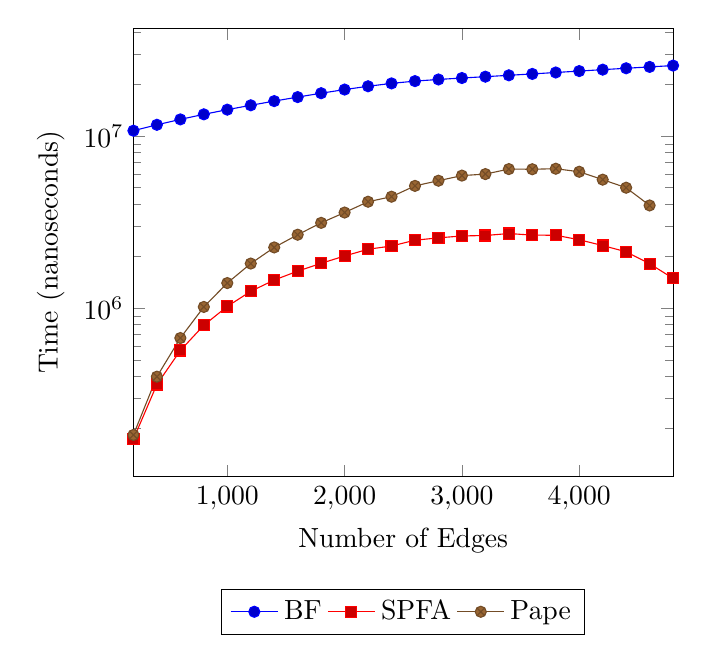
\begin{tikzpicture}
	\begin{axis}[
	ylabel={Time (nanoseconds)},
	xlabel={Number of Edges},
	ymode=log,
	xmin=200, xmax=4800,
	legend style={at={(0.5,-0.25)},
		anchor=north,legend columns=-1},
	]
	%Bellman-Ford
	\addplot+[sharp plot] coordinates
	{(200, 10733324) (400, 11613108) (600, 12487006) (800, 13361489) 
		(1000, 14224253) (1200, 15080714) (1400, 15951555) (1600, 16827772) (1800, 17725712) 
		(2000, 18613172) (2200, 19459452) (2400, 20215388) (2600, 20843340) (2800, 21307970) 
		(3000, 21722504) (3200, 22118730) (3400, 22524594) (3600, 22946628) (3800, 23391152) 
		(4000, 23838956) (4200, 24299542) (4400, 24751208) (4600, 25208962) (4800, 25662376) };
	%spfa
	\addplot+[sharp plot] coordinates
	{(200, 172802) (400, 359469) (600, 566522) (800, 793914) 
		(1000, 1021287) (1200, 1250621) (1400, 1453841) (1600, 1638197) (1800, 1819268) 
		(2000, 2006000) (2200, 2195843) (2400, 2292465) (2600, 2478774) (2800, 2556719)
		(3000, 2623366) (3200, 2638850) (3400, 2710122) (3600, 2652131) (3800, 2648458) 
		(4000, 2492793) (4200, 2306773) (4400, 2122418) (4600, 1809844) (4800, 1486166) };
	%pape
	\addplot+[sharp plot] coordinates
	{(200, 182882) (400, 398985) (600, 669097) (800, 1014356) 
		(1000, 1396380) (1200, 1813182) (1400, 2249716) (1600, 2667202) (1800, 3126314) 
		(2000, 3589348) (2200, 4147674) (2400, 4437122) (2600, 5127464) (2800, 5495913) 
		(3000, 5884082) (3200, 6005121) (3400, 6420560) (3600, 6407083) (3800, 6451954) 
		(4000, 6195652) (4200, 5573667) (4400, 5003401) (4600, 3946994) (4800, 0) };
	
	\legend{BF,SPFA,Pape}
	\end{axis}
	\end{tikzpicture}
	\caption{Edge weights are between -5 and 5}
	
	
	%-----------------
		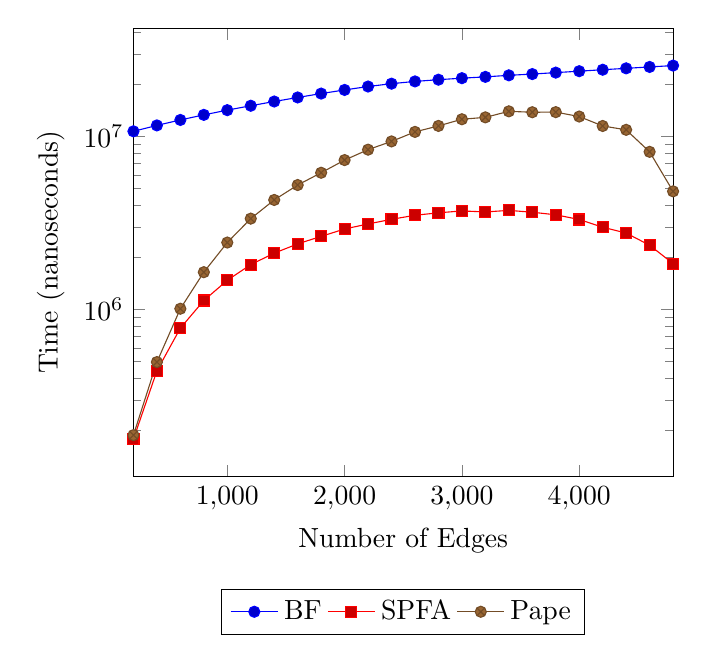
\begin{tikzpicture}
	\begin{axis}[
	ylabel={Time (nanoseconds)},
	xlabel={Number of Edges},
	ymode=log,
	xmin=200, xmax=4800,
	legend style={at={(0.5,-0.25)},
		anchor=north,legend columns=-1},
	]
	%Bellman-Ford
	\addplot+[sharp plot] coordinates
	{(200, 10735710) (400, 11614156) (600, 12489005) (800, 13364792) 
		(1000, 14229364) (1200, 15089062) (1400, 15963359) (1600, 16849198) (1800, 17739686) 
		(2000, 18625658) (2200, 19489446) (2400, 20240246) (2600, 20857690) (2800, 21344664) 
		(3000, 21775278) (3200, 22161160) (3400, 22618680) (3600, 22997654) (3800, 23449382) 
		(4000, 23899912) (4200, 24367692) (4400, 24822442) (4600, 25288468) (4800, 25755724) };
	%spfa
	\addplot+[sharp plot] coordinates
	{(200, 178363) (400, 442949) (600, 782028) (800, 1129184) 
		(1000, 1477550) (1200, 1821105) (1400, 2120059) (1600, 2400398) (1800, 2650652) 
		(2000, 2926077) (2200, 3128345) (2400, 3328069) (2600, 3512396) (2800, 3628804)
		(3000, 3720955) (3200, 3671101) (3400, 3747549) (3600, 3656643) (3800, 3533565) 
		(4000, 3319344) (4200, 2996079) (4400, 2770556) (4600, 2357327) (4800, 1845664) };
	%pape
	\addplot+[sharp plot] coordinates
	{(200, 188162) (400, 497653) (600, 1012250) (800, 1646278) 
		(1000, 2442745) (1200, 3358427) (1400, 4306396) (1600, 5251885) (1800, 6184365) 
		(2000, 7320886) (2200, 8411111) (2400, 9386805) (2600, 10652506) (2800, 11536481) 
		(3000, 12605518) (3200, 12928009) (3400, 14005389) (3600, 13841329) (3800, 13857768) 
		(4000, 13070645) (4200, 11526460) (4400, 10949119) (4600, 8169858) (4800, 4828039) };
	
	\legend{BF,SPFA,Pape}
	\end{axis}
	\end{tikzpicture}
	\caption{Edge weights are between -10 and 0}
\end{figure}



\begin{center}
	\begin{tabular}{|p{1.75cm}|p{2.25cm}|p{3cm}|p{2cm}|}
		\hline
		\multicolumn{4}{|c|}{Average Runtime Results} \\
		\hline
		Distribution	&	Algorithm	&	Max Average Runtime	Location	&	Min Average Runtime\\
		\hline
		\multirow{4}{4em}{$0 \rightarrow 10$}
			&	Bellman-Ford 		& 	(4800, 25507810) &10736436\\ 
			& 	SPFA 				& 	(4800, 675299)  &167433\\  
			& 	Pape 				& 	(4600, 731882)  &177217\\
			&	Dijkstra			&  	(4800, 358584)  &57307\\
		\hline
		\multirow{4}{4em}{$-5 \rightarrow 5$}
			& 	Bellman-Ford	& 	(4800, 25662376) &10733324\\  
			& 	SPFA 			& 	(3400, 2710122) &172802\\
			&	Pape			&  	(3800, 6451954) &182882\\
		\hline
		\multirow{4}{4em}{$-10 \rightarrow 0$}
			& 	Bellman-Ford	& 	(4800, 25755724) &10735710\\  
			& 	SPFA 			& 	(3400, 3747549) &178363\\
			&	Pape			&  	(3400, 14005389) &188162\\
		\hline
	\end{tabular}
\end{center}

The results reveal some interesting properties of the different algorithms and how they perform with sparce and dense graphs. Dijkstra's algorithm does not work with negative edges, but runs faster than GSSSP algorithms when all of the edges are non-negative. This makes sense because it is a simplier algorithm that greedily selects the next edge and never has to backtrack (or re-examine an edge). Pape ended up running slower than SPFA which was disappointing but not terribly surprising. Pape's label correction algorithm was designed to be used on SSSP algorithms so it was only included to experiment if it is valuable in a GSSSP environment. However, other label correcting algorithms, such as Bertsekas', may still be useful here.\\
The average times for Bellman-Ford stayed fairly consistent over different ranges of edge weights, but was always considerably slower than the alternative GSSSP algorithms. Also, the average times for SPFA and Pape varied considerably over the number of edges. 

\section{Next}
\subsection{Edge Iterators}
I will have to change the way I iterate over edges since, right now, it wastes time checking every potential edge. This is certainly why Adjacency List currently runs slower, even on sparse graphs. I looked into creating custom STL iterators but that would take too much time when I was near the end of the semester. Compact Star representation. I was not able to add a compact star implementation due to time constraints and other priorities but I will finish it in the future. 

\subsection{Data Structure Polymorphism}
Additionally, relating to the data structures, I wanted to change my graph generics from dynamic/run-time polymorphism (using inheritance) to static/compile-time polymorphism (templates). This proved difficult since, unlike the previous template classes I designed (algorithms and random number generator), I needed to store a container of the various template classes and didn't want to rely on using a multi-type container, such as boost::any. 
I have thought about using the curriously reoccuring template patern (CRTP) to implement different types of graphs. This would preserve relations between the different graphs and allow for some of the execution time to be move to compilation.

\subsection{Algorithms}
I wish to continue working on this project and add more algorithms and features to the generator. 

I worked on Yen's algorithm but was not able to get the algorithm working correctly. It has a lot more specific details that need to be handled. I incountered some very weird errors when working on it. For example, when iterating over the vertices in the opposite direction, the loop terminated correctly when the lower bound (since deincrementing) was $>0$. When this bound was changed to $>=0$, the loop added not 1 but 2 iterations, causing my unsigned integer to overflow during the final iteration. I tried reconstructing the loop in several different ways but encountered the same problem every time.

I would also like to implement some more label correcting algorithms to see if there are any that successfully help optimize the queue. There algorithms are very similar so it would not take longto implement more (albeit by using some duplicate code).

\subsection{Reweighting}
If there is a quick way to reweight a graph without negative cycles to have only nonnegative edges, we could run Dijkstra which is much faster than the alternative algorithms. If the cost of the reweighting preprocessing algorithm is less than the difference between cost of general SSSP and SSSP algorithms, then it would be a more efficient method to solve SSSP.

Reweighting techniques have already been seen in Johnson's all-pairs shortest path (APSP) algorithm \cite{Johnson}. Johnson's algorithm adds a new vertex that has edges of cost 0 to all other vertices. A general SSSP algorithm is run from this new vertex to find the shortest path tree. Every edge is then reweighted using:
\[c_{uv} = c_{uv} + d(u) - d(v)\]
which removes all negative edges.

\subsection{Analyzer}
I would like to build an analyzer that checks if there are any negative edges and adjusts the graph accordingly either by removing or reweighting edges. It would also check if the graph is connected from the source and removes unreached vertices. This guarentees that the graph properities, such as the number of vertices, are accurate. This also deals with not knowing many edges are in the graph when generating by probability. The analyzer also could gather detailed information about the distribution of edge weights. Since, as we saw in the results, the run-times of SPFA and Pape increased with more negative values, further research could be done to check if this is true in general. There are lots of different ways to use the distribution to perform a details analysis. For example, it could allow us to check if the run-time changes due to the raw number of negative edges, relative number of negative edges, frequency of each value or sum of all values.

\subsection{Serialization}
I would like to be able to save the graphs that are generated to create a database which lists all the properties of the graph. The database could be used to run a new algorithm to compare it to previous ones that we have tested. Instead of having to generate graphs again and running all algorithms, we would only have to run the new algorithm. This would also allow the tests to be easily and quickly repeated on different computers. 
To make sure there are no duplicate graphs in the database, a hash for each graph is created and collisions between graphs are manually compared. This way the database essentially becomes a hash table.

\begin{thebibliography}{9}

\bibitem{BF}
R.E. Bellman, \textit{On a routing problem}
Quart. Appl. Math. 16 (1958), 87-90\\
doi: 10.1090/qam/102435 

\bibitem{BF 2}
Ford Jr, Lester R. \textit{Network flow theory} No. P-923. RAND CORP SANTA MONICA CA, 1956.

\bibitem{SPFA} 
Fanding, Duan. \textit{A Faster Algorithm for Shortest-Path  SPFA} Journal of Southwest Jiaotong University 2 (1994).

\bibitem{Hu}
Hu, T. C. \textit{A decomposition algorithm for shortest paths in a network} Operations Research 16.1 (1968): 91-102. \\
doi: 10.1287/opre.16.1.91

\bibitem{Hu Torres} 
Hu, Te C., and William T. Torres. \textit{Shortcut in the decomposition algorithm for shortest paths in a network.} IBM Journal of Research and Development 13.4 (1969): 387-390.\\
doi: 10.1147/rd.134.0387
 
\bibitem{Yen1}
Yen, Jin Y. \textit{An algorithm for finding shortest routes from all source nodes to a given destination in general networks} Quarterly of Applied Mathematics 27.4 (1970): 526-530.\\
doi: 10.1090/qam/253822 

\bibitem{Yen2} 
Yen, Jin Y. \textit{Some algorithms for finding the shortest routes through the general networks.} Computing Methods in Optimization Problems-2 (1969): 377-388.

\bibitem{Yen Decomposition}
Yen, Jin Y. \textit{Technical Note—On Hu's Decomposition Algorithm for Shortest Paths in a Network} Operations Research 19.4 (1971): 983-985.\\
doi: 10.1287/opre.19.4.983

\bibitem{Bertsekas1}
Bertsekas, Dimitri P., Francesca Guerriero, and Roberto Musmanno. \textit{Parallel asynchronous label-correcting methods for shortest paths} Journal of Optimization Theory and Applications 88.2 (1996): 297-320.\\
doi: 10.1007/BF02192173

\bibitem{Bertsekas2}
Bertsekas, Dimitri P. \textit{A simple and fast label correcting algorithm for shortest paths} Networks 23.8 (1993): 703-709.\\
doi: 10.1002/net.3230230808

\bibitem{Glover1}
F. Glover, R. Glover and D. Klingman, \textit{The threshold shortest path algorithm}, Networks 14(I)
(1984). 

\bibitem{Pape}
Pape, U. \textit{Implementation and efficiency of Moore-algorithms for the shortest route problem} Mathematical Programming 7.1 (1974): 212-222.\\
doi: 10.1007/BF01585517

\bibitem{Hao}
Hao, J., and George Kocur. \textit{A Faster Implementation of a Shortest Path Algorithm} Waltham, MA: GTE Laboratories Incorporated (1992).

\bibitem{Star}
Zhou, Xin. \textit{AN IMPROVED SPFA ALGORITHM FOR SINGLE-SOURCE SHORTEST PATH PROBLEM USING FORWARD STAR DATA STRUCTURE.} International Journal of Managing Information Technology 6.1 (2014): 15.
doi:10.5121/ijmit.2014.6402

\bibitem{Dijkstra}
Dijkstra, Edsger W. \textit{A note on two problems in connexion with graphs.} Numerische mathematik 1.1 (1959): 269-271.
doi:10.1007/BF01386390

\bibitem{Johnson}
Johnson, Donald B. \textit{Efficient algorithms for shortest paths in sparse networks.} Journal of the ACM (JACM) 24.1 (1977): 1-13.
doi:10.1145/321992.321993


\end{thebibliography}

\end{document}
